\documentclass[11pt]{article}
\usepackage[margin=1in]{geometry}
\usepackage{graphicx}
\usepackage{booktabs}
\usepackage[hidelinks]{hyperref}
\title{RJ45 Insertion from Synthetic Data:\\ Dataset Surgery and Baseline Results}
\author{Parallax Worlds --- drmix campaign}
\date{August 20, 2026}

\begin{document}
\maketitle

\section{Setting}
Policies are trained on 1{,}000 simulated demonstrations (Newton physics, servo-plant
arm, Gaussian-splat rendering + Difix) of RJ45 cable insertion, and evaluated
closed-loop in the same simulator (450-step budget; success = 11\,mm insertion depth
inside a $\sim$3\,mm-tolerance bore). Three dataset variants exist on HuggingFace:

\begin{itemize}\itemsep2pt
  \item \textbf{original} (\texttt{cable\_drmix\_*}): 165{,}834 frames. The scripted
        expert decelerates to $\sim$0.02\,mm/frame at its pre-dock standoff
        ($-19$\,mm), producing near-zero action labels there.
  \item \textbf{depaused} (\texttt{*\_depaused}): arc-length resampled at a 0.2\,mm
        floor (23.1\% of frames cut, actions recomputed across cuts); no interior
        label below 0.2\,mm remains.
  \item \textbf{dp01} (\texttt{*\_dp01}): gentler 0.1\,mm floor (10.8\% cut),
        preserving the slow fine-alignment regime. Untested as of this writing.
\end{itemize}

\section{Open-loop probes (training frames)}
Per-step imitation on a training episode is near-perfect for every model
(Table~\ref{tab:probe}); open-loop metrics do not predict closed-loop behavior.

\begin{table}[h]\centering\small
\begin{tabular}{lllll}
\toprule
model & data & dpos err (mm) & direction cos & min $\lVert$pred$\rVert$ (mm) \\
\midrule
$\pi_{0.5}$ step 19999 & original & 0.088 & 0.853 & $\sim$0 at standoff \\
$\pi_{0.5}$ step 21000 & depaused & 0.096 & 0.918 & 0.212 \\
ACT c10 (15k)          & original & 0.105 & 0.800 & 0.052 \\
ACT c100 (100k)        & original & \textbf{0.037} & \textbf{0.974} & 0.031 \\
ACT c10 (15k)          & depaused & 0.146 & 0.810 & 0.148 \\
\bottomrule
\end{tabular}
\caption{Open-loop probe: first predicted action vs.\ ground truth, stride-sampled
frames of one training episode.}
\label{tab:probe}
\end{table}

\begin{figure}[h]\centering
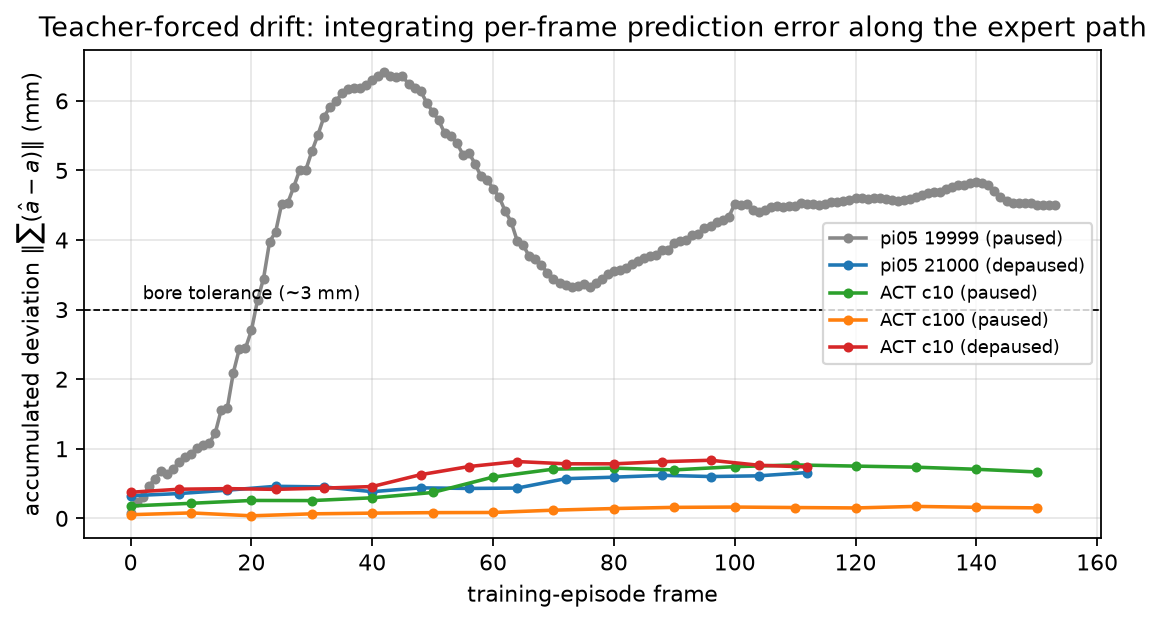
\includegraphics[width=0.78\textwidth]{openloop_drift.png}
\caption{Teacher-forced drift: accumulated prediction error
$\lVert\sum_t(\hat a_t - a_t)\rVert$ along the expert path. Only the paused
$\pi_{0.5}$ shows a large systematic bias (4.5\,mm --- the stall). Every other
model drifts $<$1\,mm \emph{when kept on the path}: the closed-loop lateral
blow-ups are not an open-loop bias, but feedback amplification of small errors
in off-path states the datasets never cover.}
\label{fig:drift}
\end{figure}

\section{Closed-loop results ($N{=}1$ per model, training-episode conditions)}

\begin{table}[h]\centering\small
\begin{tabular}{lllll}
\toprule
model & data & behavior & best position & seated \\
\midrule
$\pi_{0.5}$ 5k--20k  & original & stalls at $-19$\,mm, bounces & never enters & no \\
$\pi_{0.5}$ 21000    & depaused & drives, drifts past jack     & 4.7\,mm @ 10\,mm lat & no \\
ACT c10              & original & \textbf{slow, holds alignment} & \textbf{9.7\,mm @ 5.8\,mm lat}$^{*}$ & no \\
ACT c100             & original & blind 100-step chunks drift  & 7.8\,mm @ 10\,mm lat & no \\
ACT c10              & depaused & perfect pre-dock, then drifts & $-17.9$\,mm @ 3.0\,mm lat$^{\dagger}$ & no \\
\bottomrule
\end{tabular}
\caption{$^{*}$still advancing when the 450-step budget expired.
$^{\dagger}$best-aligned pre-dock of any run (step 40), lost during the push.}
\label{tab:closed}
\end{table}

\begin{figure}[h]\centering
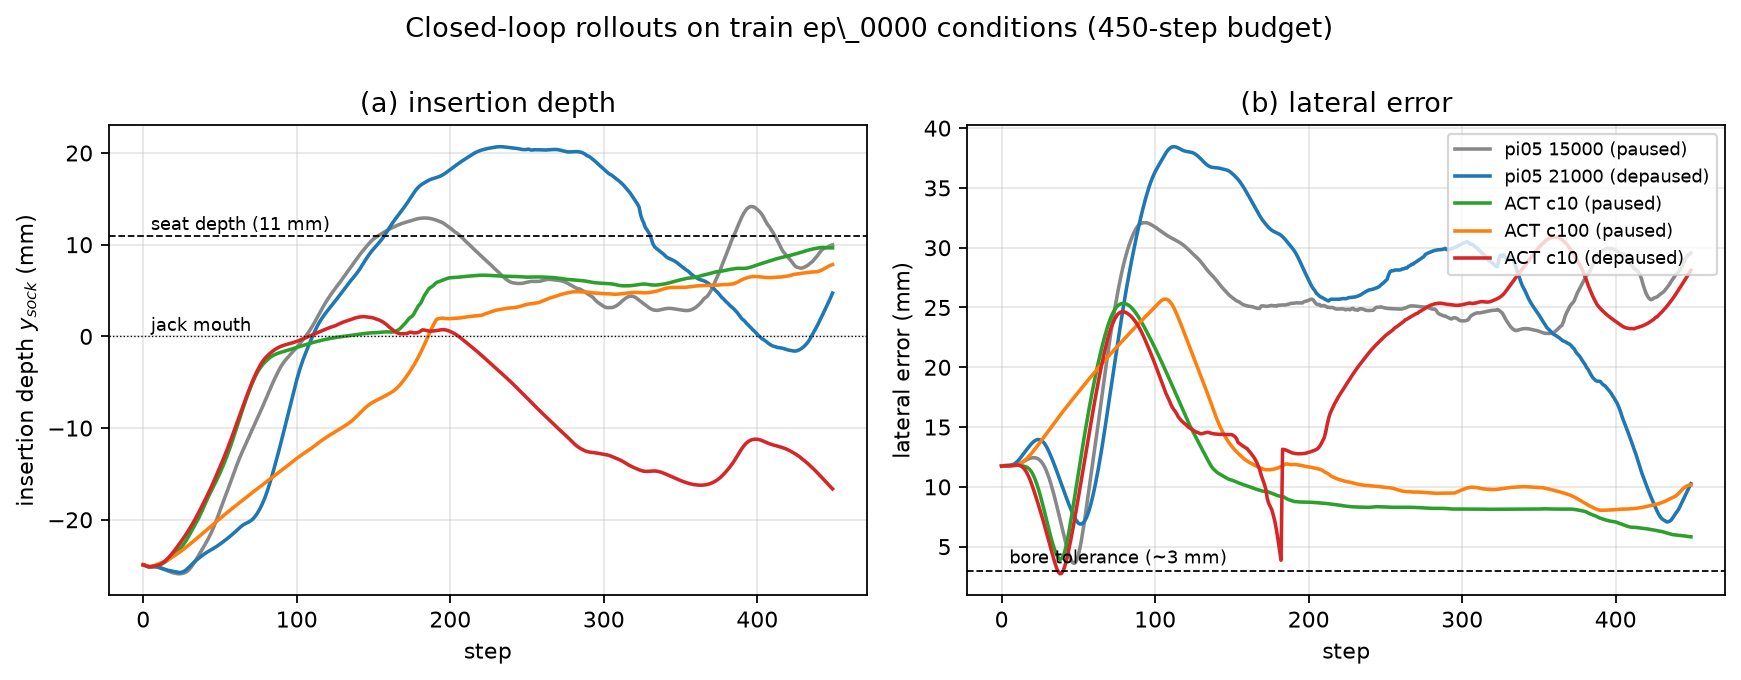
\includegraphics[width=\textwidth]{closed_loop_traces.png}
\caption{Closed-loop traces. (a) The paused $\pi_{0.5}$ never passes the pre-dock;
depaused models advance but (b) their lateral error diverges far beyond the bore
tolerance. The paused ACT c10 (green) is the only run that keeps lateral error near
tolerance while advancing.}
\end{figure}

\section{Findings}
\begin{enumerate}\itemsep2pt
  \item \textbf{The pause pathology is real but architecture-dependent.} Motionless
        pre-dock frames taught $\pi_{0.5}$ an absorbing ``output zero'' state
        (closed-loop stall). ACT, trained on the same data, averages through it.
  \item \textbf{De-pausing trades stall for imprecision.} With the 0.2\,mm floor both
        architectures move decisively but lose the slow fine-alignment behavior:
        both depaused models blow through/around the jack. Hence the gentler
        \texttt{dp01} variant.
  \item \textbf{The universal failure is uncorrected lateral drift.} Every model, both
        architectures, both datasets: once off the demonstrated path, none returns
        to it --- the datasets contain zero return-to-path demonstrations
        (classic BC compounding). Figure~\ref{fig:drift} sharpens this: on-path
        predictions are nearly unbiased ($<$1\,mm accumulated over a full episode
        for all but the paused $\pi_{0.5}$), so the failure lives entirely in
        off-path states, not in per-step accuracy.
  \item \textbf{Caveat: $N{=}1$ per model.} Failure on training conditions is a
        strong negative signal, but no rate claims are supported yet. A 40-episode
        matrix (2 models $\times$ 10 train + 10 held-out conditions) is queued.
\end{enumerate}

\section{In progress}
\textbf{Tier-2 recovery campaign} ($\sim$562 episodes, rendering): near-dock
off-nominal starts (4--16\,mm lateral, at the failure zone) and mid-flight
perturbation kicks with episodes split at the kick so only the correction is
labeled. Targets exactly the drift states above. Planned retrains: $\pi_{0.5}$
and ACT c10 on \texttt{dp01} + tier-2 recovery data.

\end{document}
